% !TEX root = main.tex
%% 这是主文件,请以此文件为主开始编排论文格式。
%% 此模板由重庆邮电大学教务处监制。
%% 编者:教务处,李茜,等;计算机学院,卢星宇,刘媛媛,等。
%% 特别感谢2022届先进制造工程学院,张治勇对初版Latex模板的大量贡献。
%% 此版由《吃胡萝卜的兔酱》进行完善,有问题可以联系2311323627@qq.com。
%% 若有任何格式错误问题或者对Latex模板的改进建议,请联系编者,欢迎各位老师同学一起完善重邮Latex模。
%% 编译指令: xelatex -> bibtex -> xelatex -> xelatex
%% overleaf: 菜单 -> 编辑器 -> xelatex 

%\special{dvipdfmx:config z 0} %取消PDF压缩,加快速度,最终版本生成的时候最好把这句话注释掉

\documentclass[UTF8,twoside,zihao=-4,AutoFakeBold,scheme=chinese,openany]{ctexbook}
% 输入配置文件,例如调用的宏包(公式,插图等)
\usepackage{graphicx} %绘图
\usepackage{pifont} %圆圈1,如①
\usepackage{booktabs} %绘制三线表
\usepackage{multirow} %使用https://www.tablesgenerator.com/网站绘制表格所需包
\usepackage{threeparttable} %表格脚注
\usepackage[noend]{algpseudocode} %绘制伪代码
\usepackage{algorithmicx,algorithm}
\usepackage{pythonhighlight} %python代码高亮
\usepackage[colorlinks=true,linkcolor=black,anchorcolor=black,citecolor=green]{hyperref}%引用参考文献、章节、图表,并跳转
\usepackage{caption}
\captionsetup[figure]{font=small,labelsep=space} 
\captionsetup[table]{font=small,labelsep=space} %图片和表格修改caption

\usepackage[final]{pdfpages}
% 设置页边距
\usepackage{geometry}
\usepackage{makecell}
\usepackage{caption}
\usepackage{multirow}
\usepackage{booktabs}
\makeatletter
\let\c@lofdepth\relax
\let\c@lotdepth\relax
\makeatother
\usepackage{subfigure}
\usepackage{float}
\usepackage[titles,subfigure]{tocloft}
\usepackage{soul}
\usepackage{color,xcolor}



\geometry{a4paper,top=3cm,bottom=2.5cm,left=2.5cm,right=2.5cm}

% 设置行间距 1.5倍
\linespread{1.5}\selectfont
% 设置段与段之间的垂直距离 \parskip默认橡皮长度是0pt plus 1pt
\setlength{\parskip}{0pt}
% \setlength{\parindent}{0pt}

%设置字体
% 设置英文字体
\setmainfont{Times New Roman}[
    BoldFont = Times New Roman Bold,
    ItalicFont = Times New Roman Italic,
    BoldItalicFont = Times New Roman Bold Italic
]

\setsansfont{Times New Roman}[
    BoldFont = Times New Roman Bold,
    ItalicFont = Times New Roman Italic,
    BoldItalicFont = Times New Roman Bold Italic
]

\setmonofont{Times New Roman}[
    BoldFont = Times New Roman Bold,
    ItalicFont = Times New Roman Italic,
    BoldItalicFont = Times New Roman Bold Italic
]

%设置字号
\usepackage{ctexsize,type1cm}
\newcommand{\yihao}{\fontsize{26pt}{39pt}\selectfont}
\newcommand{\xiaoyi}{\fontsize{24pt}{36pt}\selectfont}   
\newcommand{\erhao}{\fontsize{22pt}{33pt}\selectfont}          
\newcommand{\xiaoer}{\fontsize{18pt}{27pt}\selectfont}          
\newcommand{\sanhao}{\fontsize{16pt}{24pt}\selectfont}        
\newcommand{\xiaosan}{\fontsize{15pt}{22.5pt}\selectfont}        
\newcommand{\sihao}{\fontsize{14pt}{21pt}\selectfont}            
\newcommand{\xiaosi}{\fontsize{12pt}{18pt}\selectfont}            
\newcommand{\wuhao}{\fontsize{10.5pt}{15.75pt}\selectfont}
\newcommand{\xiaowu}{\fontsize{9pt}{13.5pt}\selectfont}    
\newcommand{\liuhao}{\fontsize{7.5pt}{11.25pt}\selectfont}

%使用公式,表格,图片
\usepackage{mathtools,amsmath,amssymb,graphicx,array,float}

% 设置页眉面脚
%% 设置章节前的页码格式
\usepackage{fancyhdr}
\fancypagestyle{content}{
	\fancyhf{}
	\renewcommand{\headrulewidth}{0pt}
	\fancyfoot[C]{\songti\xiaowu  \Roman{page}}
}

%重新设置headings
\fancypagestyle{headings}{
    \fancyhf{}
	\fancyfoot[C]{\songti\xiaowu  \Roman{page} }
	\renewcommand{\headrulewidth}{0.5pt}
	\fancyhead[CO]{\songti\xiaowu 目录 }
	\fancyhead[CE]{\songti\xiaowu 重庆邮电大学本科毕业设计(论文)}
}

%重新设置plain
%正文页眉设置
\fancypagestyle{plain}{
    \fancyhf{}
    \fancyfoot[C]{\songti\xiaowu  \thepage }
    \fancyhead[CO]{\songti\xiaowu \leftmark }
    \fancyhead[CE]{\songti\xiaowu 重庆邮电大学本科毕业设计(论文)}
}

%设置双线页脚
\makeatletter
\def\footrule{
    {\if@fancyplain\let\footrulewidth\plainfootrulewidth\fi%
    \hrule\@height 0pt \@width\headwidth          %上面0.5pt粗
    \vskip 1pt
    \hrule\@height 0pt \@width\headwidth %下面线为1pt粗
    \vskip-2\headrulewidth\vskip-1.2pt}    %两条线的距离1pt
    \vspace{8mm}}     %双线与下面正文之间的垂直间距
\makeatother

%设置文章格式
\ctexset {
    contentsname={目录},
    listfigurename={插图},
    listtablename={表格},
    figurename={图},
    tablename={表},
    bibname={参考文献},
    appendixname={附录},
    chapter={
        beforeskip={0pt},
        nameformat={\heiti\sanhao\centering},
        number={\arabic{chapter}},
        titleformat={\heiti\sanhao\centering},
    },
    section={
        format={\heiti\sihao},
    },
    subsection={
        format={\heiti\xiaosi},
    },
    subsubsection={
        format={\heiti\xiaosi},
    }
}

% 目录中的章加点
\usepackage[titles]{tocloft}
\renewcommand{\cftdot}{$\cdot$}
\renewcommand{\cftdotsep}{1.5}
\setlength{\cftbeforechapskip}{10pt}

\renewcommand{\cftchapleader}{\cftdotfill{\cftchapdotsep}}
\renewcommand{\cftchapdotsep}{\cftdotsep}
\makeatletter
\renewcommand{\numberline}[1]{%
\settowidth\@tempdimb{#1\hspace{0.5em}}%
\ifdim\@tempdima<\@tempdimb%
  \@tempdima=\@tempdimb%
\fi%
\hb@xt@\@tempdima{\@cftbsnum #1\@cftasnum\hfil}\@cftasnumb}
\makeatother

% 设置目录字体尺寸
\renewcommand{\cftchapfont}{\songti\xiaosi}
\renewcommand{\cftsecfont}{\songti\wuhao}
\renewcommand{\cftsubsecfont}{\songti\wuhao}

%使用代码排版包
\usepackage{listings}
\usepackage{color}
\lstset{%
    frame=shadowbox,
    extendedchars=false,            % 不使用xelatex而使用CJK方式处理汉字
    language=python,
    basicstyle=\sffamily,           % 设置整体格式
    keywordstyle=\bfseries,         % 关键字格式
    commentstyle=\rmfamily\itshape, % 注释格式
    stringstyle=\ttfamily,          % 字符串格式
    columns=flexible,
    escapechar=',                   % 注释中显示汉字,eg //'一个整数'
    tabsize=4,
    numbers=left,
    numberstyle=\small,             % 行号字体设置
    stepnumber=1,                   % 行号距离设置,1代表每行加行号
    numbersep=8pt,                  % 行号和代码距离设置
    backgroundcolor=\color{white},
    showspaces=false,               % show spaces adding particular underscores
    showstringspaces=false,         % 使用下划线连接字符串
    showtabs=false,
    frame=single,                   % 给代码加边框
    captionpos=b,                   % sets the caption-position to bottom
    breaklines=true,                % 自动换行设置
    breakatwhitespace=false,        % sets if automatic breaks should only happen at whitespace
    escapeinside={\%*}{*)},         % if you want to add a comment within your code
    xleftmargin=2em,                % 设置左边距,宽度默认是与页芯等宽的
    xrightmargin=2em,               % 设置右边距,宽度默认是与页芯等宽的
    aboveskip=1em                   % 设置上边距
}

%设置自定义变量
\newcommand\degree{^\cire}

% 定义文献引用格式,\cite正常引用 \supercite右上角引用
\usepackage{cite}
\newcommand{\upcite}[1]{\textsuperscript{\textsuperscript{\cite{#1}}}}
\newcommand\supercite[2][]{%
\textsuperscript{\cite[#1]{#2}}
}

\usepackage{enumitem}
\setlist[description]{
    itemsep=-5pt,
    font=\songti,
}

% 定义中文封面环境
\newenvironment{titletabbing}
{\par\bfseries\songti\sihao\tabbing}
{\endtabbing\par}

\usepackage[nottoc]{tocbibind}
\endinput


\begin{document}
\pagestyle{empty}
% 中文封面页
% !TEX root = main.tex

% 中文封面页, 不能单独编译
% 格式要求:无页眉页脚, 单独成页,后面空一页
\begin{center}
        \newcommand{\settingone}[1]{{\songti\sihao\bfseries #1}}
        \noindent {\songti\sanhao\bfseries    } \hfill
        \newlength{\Mylen}
        \settowidth{\Mylen}{\settingone{学\qquad 号:m060118xxx}}
        \begin{minipage}[t]{\Mylen} \sihao
                \bfseries 编\qquad 号 : \underline{2018123456} \\ 
                \bfseries 审定成绩 : \underline{\phantom{2018}B+\phantom{28B}} %\phantom创建空格
        \end{minipage}
         \\ [1mm]
        \newlength{\Mylentwo} 
        \begin{figure*}[h]
        	\centering
        	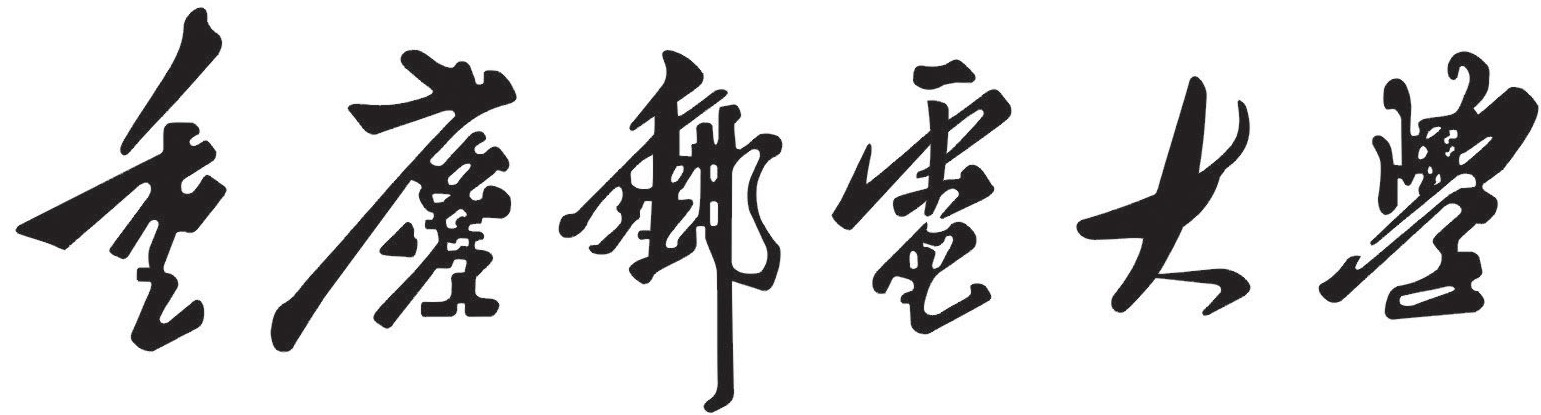
\includegraphics[scale=0.8]{images/logo/logo1.jpg}
        \end{figure*}
        %{\yihao\bfseries 重庆邮电大学} \\[3mm]
        {\yihao\bfseries 本科毕业设计(论文)}\\[3mm]
        \begin{figure*}[h]
        	\centering
        	
\includegraphics[scale=0.2]{images/logo/logo2.jpg}
        \end{figure*}

		\begin{table}[ht]
		\centering
		\renewcommand\arraystretch{1.25}
		\begin{tabular}{p{2cm}p{9cm}}
			\makecell[c]{\bfseries\sihao 中文题目}	& \makecell[c]{\bfseries\sihao 本科毕业设计(论文)写作标准} \\ 
			\cline{2-2}
			 	&  \makecell[c]{\bfseries\sihao ( 写作模板)} \\ 
			\cline{2-2} 
			\makecell[c]{\bfseries\sihao 英文题目} 	&  \makecell[c]{\bfseries\sihao Thesis Template}  \\ 
			\cline{2-2}
			&  \makecell[c]{}  \\
			\cline{2-2} 
			\makecell[c]{\bfseries\sihao 学院名称} 	&  \makecell[c]{\bfseries\sihao XXX学院}  \\
			\cline{2-2} 
			\makecell[c]{\bfseries\sihao 学生姓名} 	&  \makecell[c]{\bfseries\sihao 姓名}  \\
			\cline{2-2} 
			\makecell[c]{\bfseries\sihao 专\qquad 业} 	&  \makecell[c]{\bfseries\sihao 专业名称}  \\
			\cline{2-2} 
			\makecell[c]{\bfseries\sihao 班\qquad 级} 	& \makecell[c]{\bfseries\sihao 0231201} \\
			\cline{2-2} 
			\makecell[c]{\bfseries\sihao 学\qquad 号} 	&  \makecell[c]{\bfseries\sihao 2018123456}  \\
			\cline{2-2} 
			\makecell[c]{\bfseries\sihao 指导教师} 	&  \makecell[c]{\bfseries\sihao 姓名  职称}  \\ 
			\cline{2-2}
			\makecell[c]{\bfseries\sihao 答\hspace{6pt}辩\hspace{6pt}组} \\[-2mm] \makecell[c]{\bfseries\sihao 负\hspace{6pt}责\hspace{6pt}人} 	&  \makecell[c]{\bfseries\sihao 姓名  职称}  \\
			\cline{2-2}
		\end{tabular}
	\end{table}
	\vspace{0.1cm}
			\bfseries\sihao 2022年\hspace{12pt}6月
						\\[2mm]
						\bfseries\sihao 重庆邮电大学教务处制
\end{center}


%	\includepdf{moban.pdf} 


% 原创性声明
%% 原创性声明

%\newpage
%\begin{center}\heiti\sanhao
%
%    上海工程技术大学\\
%    学位论文原创性声明
%\end{center}

%\vspace{3em}
%
%本人郑重声明:所递交的学位论文,是本人在导师的指导下,独立进行研究工作
%所取得的成果。除文中已经注明引用的内容外,本论文不包含任何其他个人或集体已
%经发表或撰写过的作品成果。对本文的研究做出重要贡献的个人和集体,均已在文中
%以明确方式标明。本人完全意识到本声明的法律结果由本人承担。

%\vspace{5cm}
%\hspace{10cm}学位论文作者签名:

%\hspace{10cm}日期:\qquad 年 \qquad 月 \qquad 日 
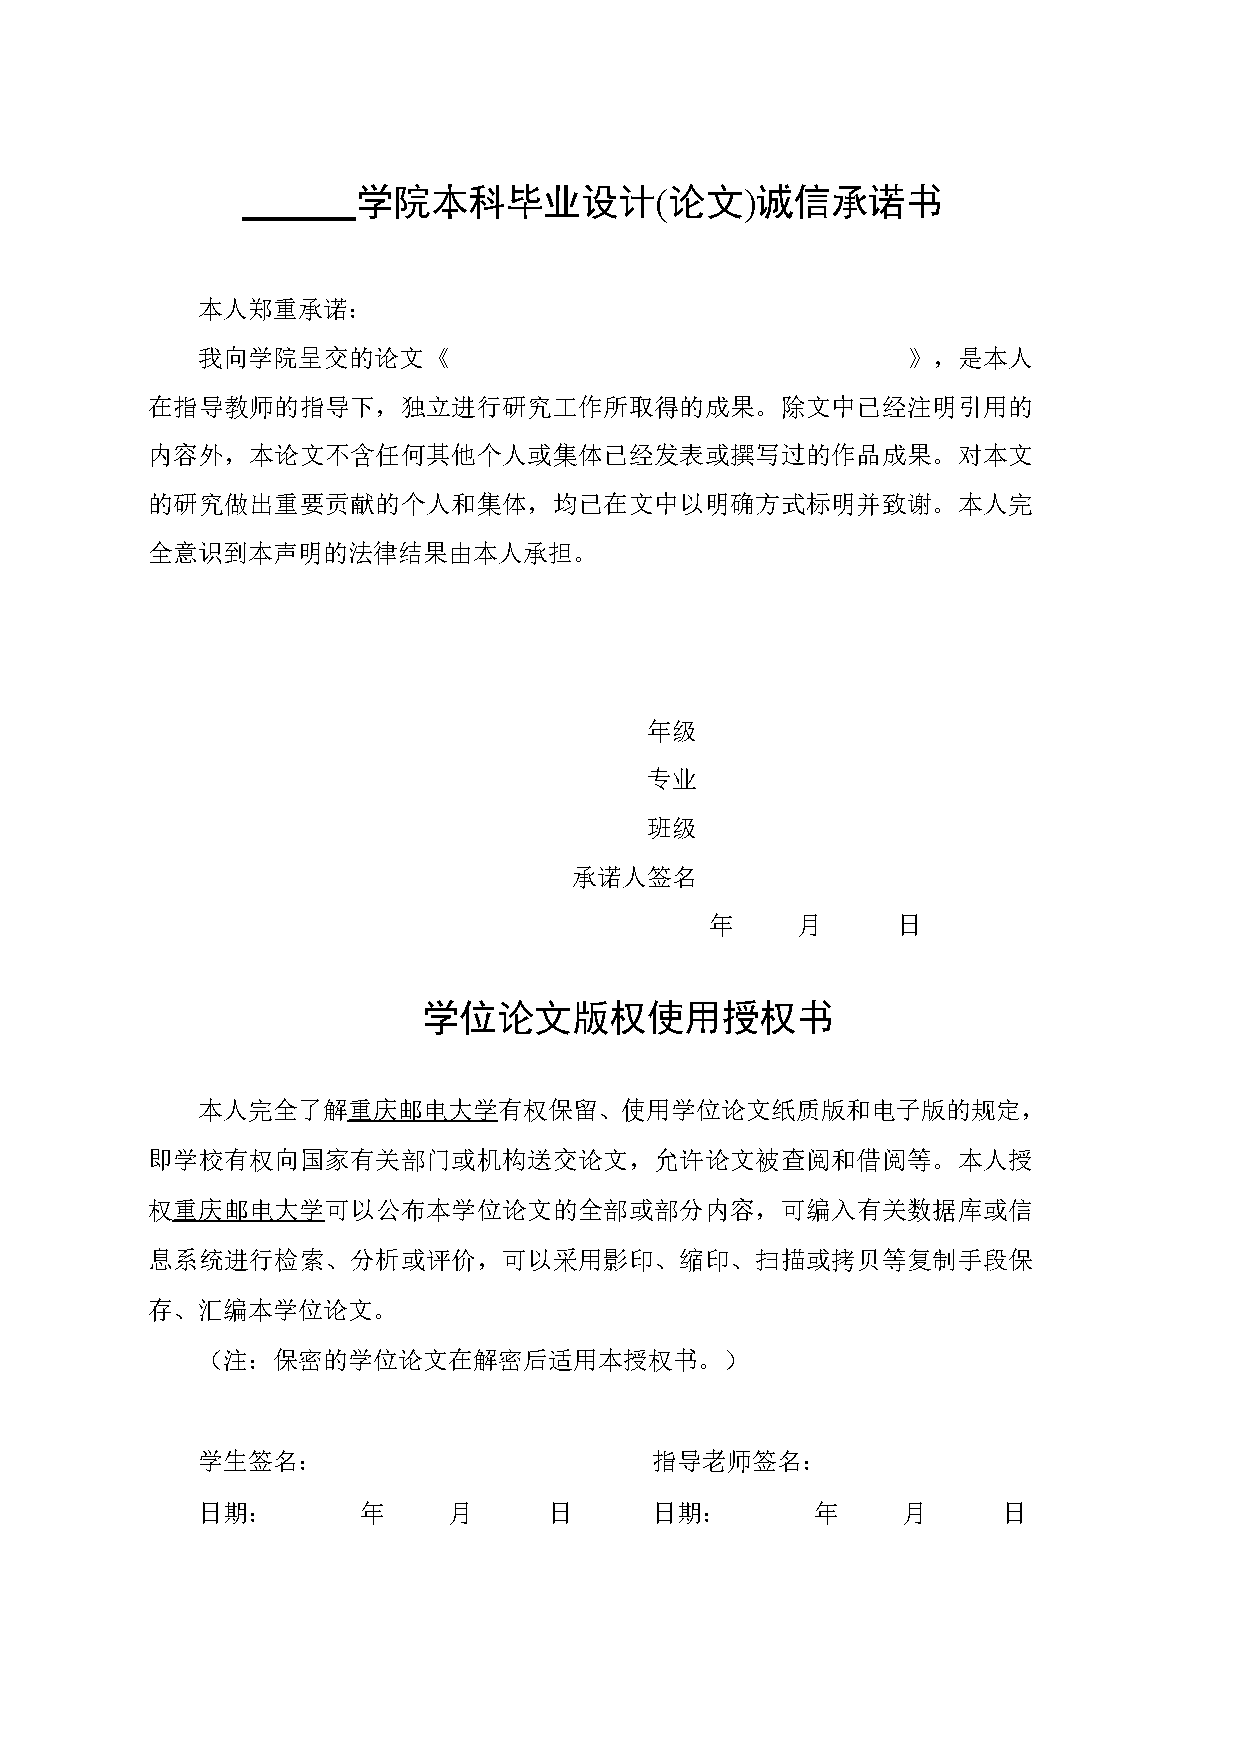
\includepdf{moban/moban2.pdf}


%% 中文摘要页,开始以罗马字母计页码
\frontmatter
\pagestyle{content}
%% 中文摘要页


\begin{center}\heiti\sanhao\textbf{
        摘要
    }
\end{center}

毕业设计是本科教学过程最后阶段的一种总结性实践教学环节。通过毕业设计,学生可以综合应用所学的各种理论知识和技能,进行全面、系统、严格的技术及基本能力的练习。为了提高毕业设计论文的质量,做到论文在内容和格式上的规范化与统一化,特制作本模板。
论文摘要是论文内容不加注释和评论的简短陈述,应以第三人称陈述,用语力求简洁、准确。中文摘要字数原则上为400-600字,英文摘要应与中文内容一致。

摘要是学位论文的浓缩,应具有独立性和自含性,即是一篇完整的短文,不阅读论文的全文,就能获得必要的信息。摘要内容应尽可能包括原论文的主要信息,包括研究工作的目的意义、主要问题、研究内容、研究方法、研究结果、主要结论,供读者确定有无必要阅读全文,也供文摘汇编等二次文献采用。摘要要用文字表达,不用图、表、化学结构式、公式、非公知公用的符号和术语。 

关键词是为了文献标引工作从论文中选取出来用以表示全文主题内容信息的单词或术语。自定义3-5个关键词,按外延由大到小排列,建议采用EI标准检索词,关键词间用逗号分开。如有可能,应尽量用《汉语主题词表》等词表提供的规范词。

“摘要”二字为黑体三号字居中,是一级标题。摘要与内容之间不空行,摘要内容与关键词间空一行。“关键词”三个字采用宋体小四号字加粗。摘要内容和关键词采用中文宋体、英文Times New Roman,小四号字,1.5倍行距。\\

\textbf{关键词:}毕业设计,论文格式,规范化,模板

\clearpage
%% 英文摘要页
%% 英文摘要页



\begin{center}\heiti\sanhao\textbf{
        Abstract
    }
\end{center}

Abstract is a brief statement of the thesis without notes and comments, which should be stated in the third person with concise and accurate language in 600-800 Chinese characters and less than 700 words in foreign languages. The writing of an abstract should follow these principles:

1. Abstract should generally state out clearly the purpose, significance, problem, methods, results, main conclusion and its significance, creative achievements and new insights of the research program, and the results and conclusions should be emphasized. 

2. Abstract should be independent and self contained, which can offer the necessary information without reading the full text. It is the miniature and abbreviation of a thesis, which contains the thesis’s main points, views and conclusions in a short and clear way. Abstract is a complete short essay with data and conclusion, which can be adopted and referred to independently. 

3. Abstract should include main information of the original thesis as far as possible for the reader to determine whether to read the full text, which can also be applied for secondary sources. 
4. Abstract should be written in words without any appended drawings and photos. Unless there is no alternative way available, abstract should be presented without graphs, tables, chemical structural equations, non-public common symbols and terminology, subscripts, and other special symbols. It is the best policy to highlight the key points clearly with less data tables.

Keywords are words or terms selected from the thesis for literature indexing to represent the topic information entry. Generally, a thesis should have 3-5 keywords, which should be arranged from broad to narrow entry according to the principle of epitaxial order. EI standard retrieval words are recommended. The keywords should be separated by a comma and there is no punctuation after the last word. If possible, it is better to use the standard words from Chinese Thesauri and other dictionaries of the same type. 

Abstract should be centered in bold-3 word size. It is the primary heading without any blank line between the word “abstract” and its content. But there should be one blank line between the abstract content and the key words. The “keywords” should be in bold Song typeface with small-four word size. The content and the key words are written in Chinese song typeface, English Times New Roman, small-four word size and 1.5 spaced.\\

\textbf{KEY WORDS:} Thesis, Format, Standardization, Template

\newpage\quad %加一页,使得目录第一页的页眉为 目录
\clearpage

%% 目录
\pagestyle{headings}
\tableofcontents
% % \thispagestyle{MyStyle}
\let\cleardoublepage\clearpage %latex消除空白页
% 符号及缩略词说明
% \thispagestyle{empty}
% \input{chapters/sym-def}
%
% ===============================
% 开始章节写作,显示特定页眉页脚
\mainmatter
\pagestyle{plain}
% 第1-7章
\chapter{引言}
\textcolor{red}{绪论(也称引言)简要说明研究工作的目的、范围、相关领域国内外研究现状、研究目标、研究设想和内容、研究和实验方法、预期结果和意义,以及论文的章节安排等。力求言简意赅,不要与摘要雷同,也不要叙述教科书中的知识。(注:每章单独另起一页。参考此格式进行排版。文中红色字体为重点要求,黑色字体仅为格式参考。)}
\section{研究背景和意义}
学位论文是学生从事科研工作的成果的主要表现,它集中表明了作者在研究工作中获得的新的发明、理论或见解,是申请学位的重要依据,也是科研领域中的重要文献资料和社会的宝贵财富。学位论文应能表明作者已在本门学科上掌握了坚实的基础理论和系统的专业知识,并对所研究课题有新的见解,有从事科学研究工作或独立担负专门技术工作的能力 \upcite{学位论文编写规则}。\textcolor{red}{(注:参考文献按照引用顺序首次出现,且文中为右上标)}

本模板主要参照《学位论文编写规则》(GB/T7713.1-2006,中国国家标准局2006年发布并实施)\upcite{学位论文编写规则}、科学出版社出版的《作者编辑手册》\upcite{汪继祥2004科学出版社作者编辑手册}、全国科学道德和学风建设宣传教育领导小组制定的《科学道德与学风建设宣讲参考大纲(试用本)》(2011年11月)\upcite{全国科学道德和学风建设宣讲教育领导小组2012科学道德与学风建设宣讲参考大纲}、《文后参考文献著录规则》(GB/T7714-2005,中国国家标准局2005年发布并实施)\upcite{曹敏2005新版《文后参考文献著录规则》解析}等制定。

部分范例来自《障碍环境中Swarm突现计算模型研究及行为控制》\upcite{王兰芬2010Swarm} 等重庆邮电大学硕士学位论文。
\textcolor{red}{(注:根据自己的课题内容,可设置若干3级目录。3级目录下按照1)→(1)→\textcircled{1}...的层次编号。)}
\section{国内外研究现状}
\subsection{国外研究现状}
\textbf{1)分类号}

分类号指中图分类号,是指采用《中国图书馆分类法》(原称《中国图书馆图书分类法》,简称《中图法》)对科技文献进行主题分析,并依照文献内容的学科属性和特征,分门别类地组织文献,所获取的分类代号。采用1999年出版的第四版《中图法》可以在http://www.33tt.com/tools/ztf(中国图书馆分类法中图分类号查询系统)或http://lib.jzit.edu.cn/sjk/tsflf/index.htm(中图法第四版计算机辅助分类查询系统)中查询。填写要求:要求分类细分到22个大类代码后三位数字。如:TN929。

\textbf{2) UDC编号	}

UDC即国际十进分类法(Universal Decimal Classification),是国际通用的多文种综合性文献分类法。UDC采用单纯阿拉伯数字作为标记符号。它用个位数(0\textasciitilde9)标记一级类,十位数(00\textasciitilde99)标记二级类,百位数(000\textasciitilde999)标记三级类,以下每扩展(细分)一级,就加一位数。每三位数字后加一小数点。如电气工程类的论文,其UDC编号为:621.3。


\subsection{国内研究现状}
论文中文题名是以最恰当、最简明的词语,反映学位论文最重要的特定内容的逻辑组合。题名用词应有助于选关键词和编制题录、索引等二次文献,可以提供检索的特定实用信息。题名应恰当简洁,一般不超过25个字。题名应避免使用不常见的缩写词、首字缩写字、字符、代号及公式等。题名语意未尽时,可以用副标题补充说明论文中的特定内容[1]。题名中文宋体,英文Times New Roman小二号字。


\section{主要内容和工作安排}
写出论文的主要工作内容,并逐一介绍每章的内容安排。全文共分为5章,内容结构安排如下:

第1章为引言,引入课题的研究背景及意义….

第2章是天线基本理论分析,….

第3章是设计仿真,….

第4章为优化与分析,….

第5章作为论文的结束语,总结毕业设计工作,提出可以在今后继续深入研究的方向。



\chapter{论文结构及文字格式}
学士学位论文应能表明作者确已较好地掌握了本门学科的基础理论、专门知识和基本技能,并从事科学研究工作或独立担负专门技术工作的初步能力。论文的文字表述应实事求是、客观真切、合乎逻辑、层次分明、简练可读。凡引用他人观点、方案、资料、数据、图表等,无论是纸质或电子版,均应详加注释。论文结构和文字格式应规范。\textcolor{red}{(注:参考此格式进行排版。标题名称,自己根据情况进行修改。)}
\section{论文结构}
论文由前置部分、主体部分和附录部分构成。前置部分包括封面、封二、中英文摘要、中英文关键词、目录、图录、表录、注释表、附件清单等;主体部分包括引文、正文、结论、致谢、参考文献等;附录部分为论文主体部分的补充,用于编排论文相关的资料,如设计说明、软件源代码、设计图纸、测试报告、英文翻译等。

论文应根据内容的相对独立性划分各章,每章的内容精简后可作为期刊论文发表,各章的顺序安排应考虑论文内容的逻辑性。各章之间应重新分页,章的标题在起始页。

论文正文是论文的核心部分,占主要篇幅。由于研究工作涉及的学科、选题、研究方法、工作进程、结果表达方式等有很大差异,对正文内容不作统一规定,但正文应对研究内容及成果进行较全面、客观的理论阐述,应着重指出研究内容中的创新、改进与实际应用之处。


\section{学位论文中的引言}
\subsection{引言的目的}
国家标准GB7713-87规定:引言(或绪论)简要说明研究工作的目的、范围、相关领域的前人工作和知识空白、理论基础和分析、研究设想、研究方法和实验设计、预期结果和意义等。应言简意赅,不要与摘要雷同,不要成为摘要的注释。一般教科书中有的知识,在引言中不要赘述。

学位论文需要反映出作者确已掌握了坚实宽广的基础理论和系统深入的专门知识,具有开阔的科学视野,对研究方案作了充分论证,因此,有关历史回顾和前人工作的文献综述,以及理论分析都可以放在引言里。

引言的目的是给出作者进行本项工作的原因,希望达到的目的。因此应给出必要的背景材料,让对这一领域并不特别熟悉的读者能够了解进行这方面研究的意义,前人已达到的水平,已解决和尚待解决的问题,引出要研究的内容,介绍通过研究取得的成果和主要创新之处。



\subsection{引言构成及写作要求}
引言的构成及写作要求如表~\ref{tab:2.1}所示。\textcolor{red}{(点表2.1可以跳转到该表)}


\begin{table}[h] %htbp 可以调整图或表的位置
    \small       %设置字号五号 
	\centering
	\caption[表2.1]{引言构成及写作要求}
	\label{tab:2.1}
    	\begin{tabular}{m{7cm}|m{7cm}}
    	\hline 
        \makecell[c]{\textbf{基本项目}} 	&\makecell[c]{\textbf{主要内容}}\\ 
        \hline 
        研究的必要性(存在的问题)	& 原来存在的问题,提出了什么要求,说明这项研究的意义 \\ 
        \hline 
        历史的回顾	&  对于存在的问题,前人进行过怎样的研究,介绍其大概情形\\ 
        \hline 
        前人研究中存在的欠缺	& 考察了前人的研究之后,发现了什么欠缺,还可以介绍自己研究的动机 \\ 
        \hline 
        写作论文的目的和作者的想法	& 写作目的和涉及的范围,研究结果的适用范围,研究者有什么建议,研究的新特点是什么 \\ 
        \hline 
        处理方法和研究结果简介(具体数据)	& 引用从具体数值计算出的数据,介绍研究的经过和结果 \\ 
        \hline 
        \end{tabular} 
\end{table}




\section{本章小结}
本科毕业论文由前置部分、主体部分和附录部分构成,撰写论文时需按此模板要求和格式编排。


\chapter{注释、图表、公式和计量单位格式}
论文中常常要用注释、图表、公式和计量单位表达研究工作内容。除了要注重论文结构的规范性,规范的注释、图表、公式和计量单位格式同样是论文质量的基本保证。\textcolor{red}{(注:认真阅读本章内容,图、表、公式等,参考此格式进行排版。)}
\section{注释}
注释是正文中为了不中断或割离连贯的叙述语言而对文中某些内容(如词语、内涵、引文出处、资料来源等)加以必要说明的文字。在论文写作中常用到的注释有注释表、脚注、图注和表注。注释表是指论文中符号、标志、缩略词、首字母缩写、计量单位、名词、术语等的注释汇集说明。这些文字按页排在页下方的叫脚注;排在图题下方或表格下方的叫图注或表注,这些都放在正文中。

脚注用6号字排在相应正文同一页最下部。脚注按在同一页中出现的先后,在被注文字右上角依次编排序号,如\textcircled{1}、\textcircled{2}…。序号标示位置应紧靠被注文字,若被注文字后紧跟有标点符号,当此标点是顿号和逗号时,注序号放在标点符号前;其他标点符号,应根据被注释内容确定放在标点符号之前或之后。注文的序号应与文中所注序号相同。注文与正文之间用脚注线(细线,顶格排,长约版心宽度的四分之一)隔开。各条注文单列,均缩进两格起排,转行顶格,句末加句号。同一页正文中出现相同内容的注释时,第二次及其以后序号应与第一次相同,不必再顺序编号和重复加注文[2]。脚注的示例见1.3节。图注和表注的具体用法在~\ref{section:3.2}节中介绍。



\section{图表格式}
\label{section:3.2} %这里是章节的标签,引用时需要
\subsection{图格式}
图包括曲线图、构造图、示意图、图解、框图、流程图、记录图、布置图、地图照片、图版等。学位论文的插图、照片必须确保能复制或微缩,以矢量图为最佳,且原则上应使用矢量图(尤其是来源本来就是图形工具绘制的矢量图)。

图应有“自明性”,即只看图、图题和图注,不阅读正文,就可以理解图意。如图~\ref{fig:3.1}所示\textcolor{red}{(点图3.1可以跳转到该图)},图应编排序号。图的编号一律用阿拉伯数字依序连续编排,序号分章依序编号,其标注形式应便于互相区别,例如:图1.1、图1.2、图3.1、图3.2等。每一章图的编号应连续。如某章只有一幅图时,仍应标为“图×.1”。

图要有图题,是简短确切的题名,中文字体为宋体5号字,并置于图的编号之后,图的编号和图题应置于图下方的居中位置。
% LaTex图片的插入与引用 
% 参考:https://blog.csdn.net/liudongdong19/article/details/118362085
\begin{figure}[htbp]
	\centering
	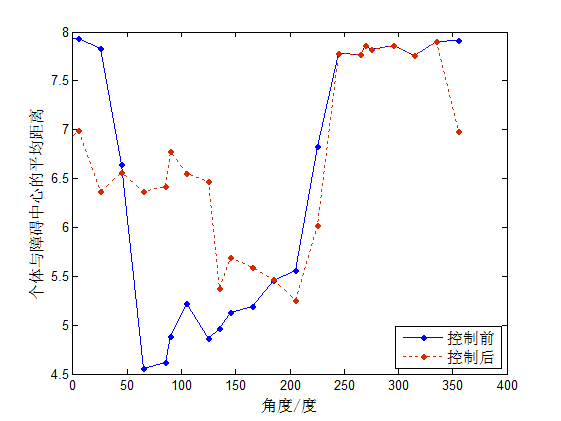
\includegraphics[width=10cm]{images/chapters/3.1}
	\caption{不同躲避角度下的Swarm-MAD模型群体与障碍中心平均距离\upcite{王兰芬2010Swarm}} 
	\label{fig:3.1} 
\end{figure}

必要时,图还要有图注。图注指对图中的符号、标记、代码,以及实验条件等项目作补充说明或解释的简明文字。当插图的图元过多而不方便用文字注释时,在图中改用图元代号(往往用外文字母的大小写或正斜体、数字来表示不同系列的代号);在图外,即图题下放置图元代号的说明(即图注)。图注通常排在图题下方。图注的字号为6号。注释或说明图中项目时,其符号、阿拉伯数字、外文字符等,必须与图中一一对应。并列注释时,各项目通常用分号分开;句子较长,或一项注释中已有分号或句号时,各项间只能用句号分开,不能再用分号。图注应编排序号,注的序号以同一页内出现的先后次序单独排序,用\textcircled{1}、\textcircled{2}、\textcircled{3}…依次标示在需加注处[2]。

图与图题与正文之间空一行。分图题置于分图之下,分图号用(a)、(b)等表示,图3.2和图3.3为包含分图的图设置规范。图应居中,容易出现问题是图所在行出

图与图题与正文之间空一行。分图题置于分图之下,分图号用(a)、(b)等表示,图3.2和图3.3为包含分图的图设置规范。图应居中,容易出现问题是图所在行出现缩进,而导致图没有真正居中。多图要均匀排列,可利用虚框表格控制格式,如图3.2。

\begin{figure}[htbp]
	\centering
	\subfigure[平均个体聚类度变化图]{
    	\label{fig:3.2a}
		\begin{minipage}[t]{0.5\linewidth}
		 \centering
			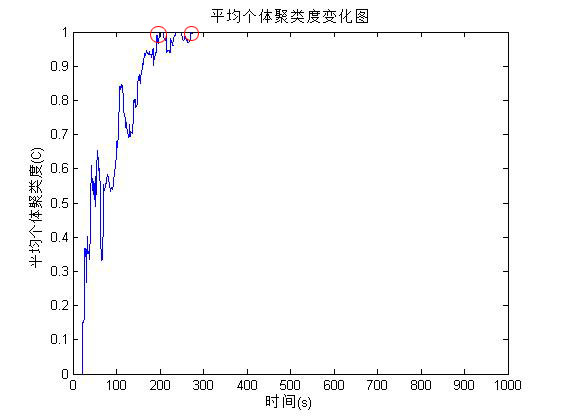
\includegraphics[width=7cm]{images/chapters/3.2a} 
		\end{minipage}%b
	}%
	\subfigure[邻域个体分布指数变化图]{
	    \label{fig:3.2b}
		\begin{minipage}[t]{0.5\linewidth}
			\centering
			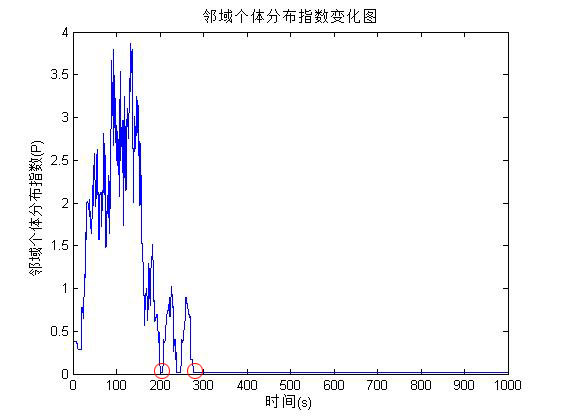
\includegraphics[width=7cm]{images/chapters/3.2b} 
			%\caption{fig2}
		\end{minipage}%
	}%
	\centering
	\caption{标示群体突现时刻的指标变化图\upcite{王兰芬2010Swarm}}
	\label{fig:3.2}
\end{figure}

\begin{figure}[htbp]
	\centering
	\subfigure[θ = 0°(原模型)]{
    	\label{fig:3.3a}
		\begin{minipage}[t]{0.5\linewidth}
		\centering
		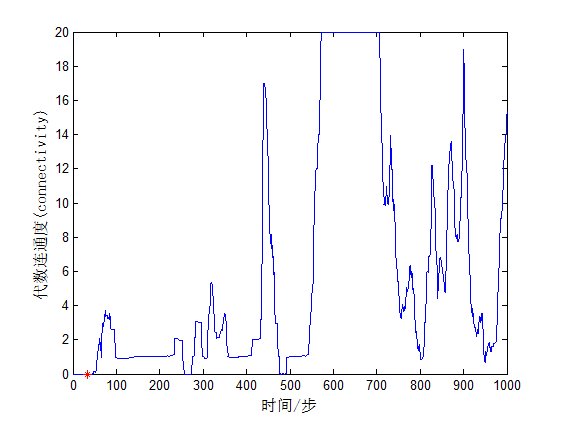
\includegraphics[width=7cm]{images/chapters/3.3a}
		\end{minipage}%b
	}%
	\quad  %空格
	\subfigure[θ= 5°,25°,45°]{
	    \label{fig:3.3b}
		\begin{minipage}[t]{0.5\linewidth}
		\centering
		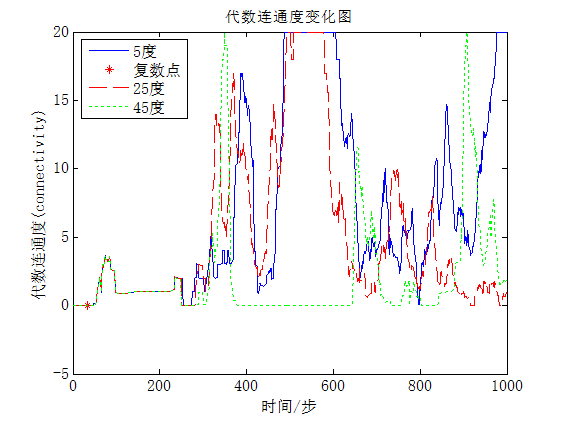
\includegraphics[width=7cm]{images/chapters/3.3b}
		\end{minipage}%
	}%
	\centering
	\caption{标示群体突现时刻的指标变化图\upcite{王兰芬2010Swarm}}
	\label{fig:3.3}
\end{figure}

曲线图的纵横坐标必须标注“量、标准规定符号、单位”。此三者只有在不必要标明(如无量纲等)的情况下方可省略。坐标上标注的量的符号和缩略词必须与正文一致。

照片图要求主题和主要显示部分的轮廓鲜明,便于制版。如用放大缩小的复制品,必须清晰反差适中。照片应有表示物尺寸的标度。

引用图应在图注中标出文献资料来源。

文中必须有关于本插图的提示,如“见图1.1”、“如图1.1所示”等。该页空白不够排写该图整体时,则可将其后文字部分提前排写,将图移到次页。

可以根据图的大小,将两个图并列放置,如图3.4和图3.5所示。


\begin{figure}[htbp] 
	\begin{minipage}[t]{0.5\linewidth} 
		\centering 
		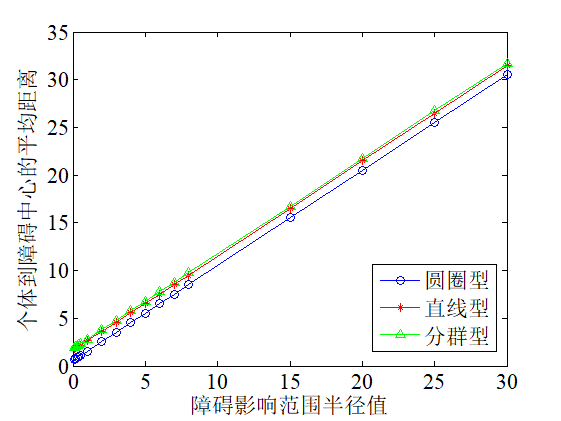
\includegraphics[width=7.5cm]{images/chapters/3.4} 
		\caption{个体与障碍中心平均距离\upcite{王兰芬2010Swarm}} 
		\label{fig:3.4} 
	\end{minipage}% 
	\begin{minipage}[t]{0.5\linewidth} 
		\centering 
		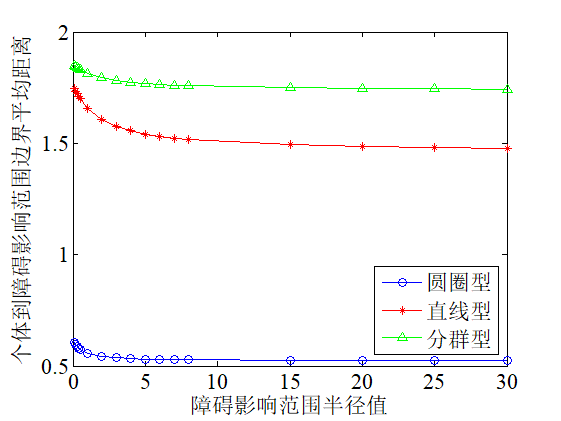
\includegraphics[width=7.5cm]{images/chapters/3.5} 
		\caption{个体到障碍影响范围边界平均距离\upcite{王兰芬2010Swarm}} 
		\label{fig:3.5} 
	\end{minipage} 
\end{figure}


\subsection{表格式}
表的编排一般是内容和测试项目由左至右横读,数据依序竖读。表应有自明性。表应编排序号,编号方式与图编号方式相同。例如:表1.1、表1.2、表3.1、表3.2等。

表要有表题,是简短确切的题名,并置于表的编号之后,表的编号和表题应置于表上方居中位置。必要时,应将表上的符号、标记、代码,以及需要说明事项等,用最简练的文字,横排于表题下,作为表注。表注应编排序号,与图注相同。

表注主要包括三种情况:资料来源(说明表中数据的文献来源,可用标题上引用参考文献、表下说明出处或脚注三种方式之一给出)、普通注解(对表中的数据处理的说明)、特殊注解(对某一个或几个表栏项目进行特别说明),如表3.1所示。表注通常用与表格内容相同的字体字号排在表格下方。表注的标号既可以表题与表内连续编号,用\textcircled{1} \textcircled{2}…标注在被注文字的右上角,也可以表题用“注:”或“*”号,表内用\textcircled{1} \textcircled{2}…分别编序号。无论采用哪种形式,全文要统一[2]。其中,采用参考文献引用方式时,该参考文献应符合参考文献要求(具体见第6章规定)。如仅引用少量内容,和本文工作相关度不大,应采用另外两种方式给出出处。

\begin{table}[t]
	\centering
	\small %保证表内字号为五号
	\caption[表3.1]{电流类型对效率的影响}
	\label{tab:3.1}
	\begin{threeparttable}
    	\begin{tabular}{m{4cm} m{3cm} m{3cm} m{3cm}}
    		\hline 
    		\makecell[c]{\textbf{电流类型}} & & & \makecell[c]{\textbf{$\frac{{{n_g}}}{\% }$}}\\ 
    		\hline 
        	\makecell[c]{${J^2}(t) = 1$}	&\makecell[c]{4.27}  & \makecell[c]{1.28} & \makecell[c]{43.9(30)}\\ 
    		\makecell[c]{${J^2}(t) = 1$}	&\makecell[c]{4.64}  & \makecell[c]{1.39} & \makecell[c]{41.8(29)}\\ 
        	\makecell[c]{${J^2}(t) = \frac{1}{t}$}	&\makecell[c]{3.28}  & \makecell[c]{0.98} & \makecell[c]{50.5}\\
    		\hline 
    	\end{tabular} 
    	\begin{tablenotes}
            \footnotesize
            \item[*] 资料来源:Wang Ying et al.2004.Physics of Electric Launch.Science Press。%星号*可以换成数字或是其他的字符
         \end{tablenotes}
     \end{threeparttable}
\end{table}

文中必须有关于表的提示,可用“见表1.1”、“如表1.1所示”等。如“两种模型应用下球队与UVA球队的比赛结果如表3.2所示。”

\begin{table}[htbp]
    \centering
    \small
	\caption[表3.2]{球队的比赛结果统计表\upcite{王兰芬2010Swarm}}
	\label{tab:3.2}
	\begin{tabular}{cccccc}
		\hline
		\multirow{2}{*}{模型}       & \multirow{2}{*}{d} & \multirow{2}{*}{r} & \multirow{2}{*}{与对方队员的警戒距离} & \multicolumn{2}{c}{改进球队 VS UVA球队} \\ \cline{5-6} 
		&                    &                    &                             & 比分           & 拿球进攻时间      \\ \hline
		\multirow{4}{*}{Swarm}    & 10.0               & 5.0                &              & 0:6          & 3978:2014 \\ 
		& 30.0               & 10.0               &                             & 0:4          & 2754:3010          \\ 
		& 50.0               & 10.0               &                             & 0:5          & 3174:2806          \\  
		& 70.0               & 10.0               &                             & 0:0          & 3113:2856          \\\hline
		\multirow{3}{*}{Swarm-OA} & 70.0               & 10.0               & 10.0                        & 1:2          & 3132:2794          \\
		& 70.0               & 10.0               & 70.0                        & 0:3          & 3180:2772          \\
		& 70.0               & 10.0               & 50.0                        & 0:1          & 2858:3012         \\ \hline
	\end{tabular} 
\end{table}

表名中不允许使用标点符号,表名后不加标点。表名与正文之间空一行。数字空缺的格内加横线“-”(占2个数字宽度)。

表内文字或数字上、下或左、右相同时,采用通栏处理方式(合并单元格),表内文字或数字上、下或左、右相同时,采用通栏处理方式(合并单元格),或一律填上具体数字或文字,不允许用“〃”、“同上”之类的写法。

表内文字说明,起行空一格、转行顶格、句末不加标点。

表的各栏应标明“量、标准规定符号、单位”。此三者只有在不必要标明(如无量纲等)情况下方可省略。表中的缩略词和符号,必须与正文一致。

如某个表需要转页接排,在随后的各页上应重复表的编号。编号后跟表题(可省略)和“(续)”,如“表1.1 xxxx(续)”或“表1.1(续)”所示,续表均应重复表头和关于单位的陈述。编号后加“(续表)”,表题可省略。续表应重复表头[2]。
 
表格不加左、右边线。表的编排建议采用国际通行的三线表或不完全表。其中,三线表通常只有3条线,即顶线、底线和栏目线,没有竖线,以其形式简洁、功能分明、阅读方便而在科技论文中被推荐使用,如表3.1和3.2。不完全表是指有其余表线,没有左右两根边线的表格,如表2.1和表2.2(为区别表内容和表头,此时表头文字可加粗)。可根据内容采用两种形式之一,以形式简洁但不带来阅读者理解困难为前提。附录A使用了常见的完全表(即所有表线不省略)。

表题、表内文字和表注一般均为宋体5号字,单倍行距。根据内容多少,为保证一行排版,也可适当减小字号或紧缩字体排版。表中单元格的间距合适,紧促美观。

\section{公式格式}
正文中的公式、算式或方程式等应注明编号,按章顺序编排,公式的编号右端对齐(当有续行时,应标注于最后一行),公式与编号之间用空格连接。公式中字符大小合适,基本字符大小与正文匹配,为小4号。即一个变量在正文中是小4号,那么公式中显示效果与之一致,也应为小4号字体,上、下标等字符等参照此字号减小。

公式应另起一行居中排,公式较长时最好在等号“=”处转行,如难实现,则可在+,-,×,÷,<,>等运算符号处转行,转行时运算符号仅书写于转行式前,不重复书写。上下式在符号“=”处对齐。

公式中第一次出现的物理量代号应给予注释,注释的转行应与破折号“——”后第一个字对齐。破折号占二个字,注释物理量需用公式表示时,公式后不应出现公式序号。公式下面的“式中”空两个字起排,单独占一行。公式中所要解释的符号按先左后右,先上后下顺序分行空两个字排,再用破折号与释文连接,回行时与上一行释文对齐。上下行的破折号对齐。

公式中应注意分数线的长短(主、副分数线严格区分),长分数线与等号对齐。


示例1:
\begin{equation}
    \label{equ:3.1}
    a = {a_{\max }}\frac{v}{{\left| v \right|}} %使用~\ref{equ:3.1}引用公式
\end{equation}

\textcolor{red}{其中:(注:留意此段不应缩进,和上行属于同一段。这是论文常见问题。)}

\begin{equation}
v = {c_1}{v_1}(d) + {c_2}{v_2}(d) + {c_3}{v_3}(d) + {c_4}{v_4}(d) + {c_5}{v_5}(d) \label{gongshi3.2}
\end{equation}

式中,$ c_{1}~c_{5}$——各项的权值,常数

     \hspace*{1.1cm}  ${v_r}$——单位随机向量
     
     示例2:
     
     {\large $x = \frac{{2\pi ({n_1} + {n_3})}}{{\frac{{{n_1} + {n_2}}}{{{n_1} - {n_2}}}}}$}
     
     
\section{计量单位格式}

文中所用的物理量和单位一律采用《中华人民共和国法定计量单位》,并遵照《中华人民共和国法定计量单位使用方法》(GB3100~3102-93)。单位名称和符号的书写方式一律采用国际通用符号,全文统一。物理量用斜体,单位用正体。

\section{本章小结}

介绍了论文中出现的注释、图表、公式和计量单位的格式,以及在图表中注释,即图注和表注的标注方法,供撰写论文时参照执行。 

\newpage\quad %加一页,使得第四章第一页的页眉为 第四章标题

\chapter{其他格式要求}

学位论文中对其他的格式要求还要页面要求、页眉页脚要求、正文的层次安排、打印要求和论文查非要求等。\textcolor{red}{(注:仅参考此格式进行排版。)}

\section{页面要求}

学位论文用A4(210×297mm)纸,采用双面打印,装订成品尺寸:207×291mm。

论文外部封面采用学校当年统一印刷提供的封面。此论文模板封面为内封,应是打印论文时的内页首页。评审、答辩等中间环节提供的纸质论文可不用学校统一外封面正式装订,而是用本模板封面作为临时封面。

\section{页眉}

从目录页开始到论文最后一页,均需设置页眉。页眉内容:\textcolor{red}{偶数页居中对齐为“重庆邮电大学本科毕业设计(论文)”,奇数页居中对齐是各章章名;}字体采用宋体5号。页眉之下有一条下划线。\textcolor{red}{封面、摘要没有页眉,也没有边框。}

\section{页脚}

页脚放置页码,页码在版芯下边线之下隔行居中放置;摘要、目录、图录、表录、注释表等文前部分的页码用罗马数字单独编排,正文以后,从引言开始的页码用阿拉伯数字连续编排。

\section{打印要求}
\subsection{页面设置}

学位论文页边距按以下标准设置:上边距(天头)3厘米,下边距(地脚)2.5厘米,左右边距2.5厘米,装订线靠左1厘米,页眉顶端距离1.6厘米,页脚底端距离1.5厘米。无网格。

\subsection{字体}

论文正文的中文字体用宋体;英文字体则要求为Times New Roman。正文中的文字部分要求两端对齐。

\subsection{字号}

1)目录题目(目录、图录、表录、注释)——是一级标题,中文黑体、英文Times New Roman, 3号字居中,段前17磅,段后16.5磅,1.5倍行距;

2)章标题(第x章)——是一级标题,中文黑体、英文Times New Roman, 3号字居中,段前17磅,段后16.5磅,1.5倍行距;

3)节标题(x.x)——是二级标题,中文黑体、英文Times New Roman小3号字顶格居左,段前13磅,段后13磅,1.5倍行距,节名和文字间空1个字符,不空行;

4)条标题(x.x.x)——是三级标题,中文黑体、英文Times New Roman4号字顶格居左,段前13磅,段后13磅,1.5倍行距,条名和文字间空1个字符,不空行;

5)正文——中文宋体、英文Times New Roman小4号,首行缩进2字符,1.5倍行距;

6)正文后的题目(参考文献、致谢、攻读xx期间发表的论文)——是一级标题,中文黑体、英文Times New Roman, 3号字居中,段前17磅,段后16.5磅,1.5倍行距。


\section{论文查重要求}

为进一步提高我校本科毕业(设计)论文教学质量,加强规范管理,科学引用文献资料,树立良好学风,防止本科毕业(设计)论文抄袭、拷贝、篡改已有科研成果等学术不端现象的发生,学校决定使用“大学生论文抄袭检测系统”对毕业生的毕业(设计)论文进行检测。

\textbf{1)检测范围}

毕业(设计)论文均可通过“维普论文检测系统”进行检测,各学院可根据本学院各专业的实际情况设定本科毕业(设计)论文进行检测的抽查规则,但抽检的论文占总人数的比例不得低于45\%。

维普论文检测系统网址:http://vpcs.cqvip.com/login.aspx?sysid=2

\textbf{2)检测标准}

检测结果中,毕业(设计)论文文字复制比(即毕业(设计)论文的某一章节与比对文献比较后,重合文字部分在该章节中所占的比例)在30\%(含30\%)以内的视为合格,文字复制比超过30\%的视为不合格。参评校级优秀毕业(设计)论文必须经过检测并且复制比应控制在20\%以内。

\textbf{3)检测不合格处理}

检测不合格的毕业(设计)论文,给予一次修改机会,经再次检测合格后方可申请答辩与成绩评定;复检仍不合格的延期答辩。

\section{论文非学术性错误}
论文中的非学术型错误主要包含错别字、格式错误、图表错误、参考文献格式错误、序号列表错误、排版问题等被普遍认为的非学术型的低级错误。论文中存在大量低级错误,说明论文写作质量差,影响读者对其学术水平的判定,同时也反映了该论文作者缺乏认真、严谨、负责的科学态度和素养,没有达到合格人才的培养目的。学位论文写作中非学术性错误的主要表现见附录A。

\section{本章小结}
介绍了学位论文的其他格式要求,以及学校关于检查论文中非学术性错误(俗称低级错误)的要求。

\newpage\quad %加一页,使得第五章第一页的页眉为 第五章标题







\chapter{科学道德与学风}

学位论文撰写时要遵循科学道德,树立良好学风。本章介绍科学道德与学风中和学位论文撰写密切相关的四个方面,在撰写学位论文时要拒绝科研不端行为,规避科研不当行为,注意科研规范和引文规范。\textcolor{red}{(注:仅参考此格式进行排版。)}

\section{科学道德与学风问题}

科学道德与学风问题是指科技工作者在科研规范、行为准则、治学精神、治学态度、治学风气、治学原则等方面出现的失范现象。反映了现代科研体制在科研活动中存在的问题和漏洞,既有科技工作者精神层面的伦理道德问题,也有行为层面的科研规范问题[3]。

中国科协《科技工作者科学道德规范(试行)》规定的违反科学道德的学术不端行为主要表现为七种类型,具体描述见附录B。

\section{科研不端行为}

本节内容均摘自文献[3],后文未一一引用。

\subsection{科研不端行为的定义}

国际科技界将严重违反基本的科学诚信的行为称为科研不端行为(misconduct in science,或称scientific misconduct),这种行为与科研违规行为、科研越轨行为的内涵十分接近。科研不端行为主要有以下三方面特征:第一,违反科学界通用的道德标准,或严重背离相关研究领域的行为规范;第二,不端行为是蓄意的、明知故犯的或是肆无忌惮的;第三,不端行为不包括诚实的错误或者观点的分歧。

综上所述,科研不端行为的理解如图5.1所示。

2007年,中国科学院发布《中国科学院关于加强科研行为规范建设的意见》,明确将科研不端行为进行定义,并分为以下几类:

1)在研究和学术领域内有意做出虚假的陈述,包括:编造数据;篡改数据;改动原始文字记录和图片;在项目申请、成果申报,以及职位申请中做虚假的陈述。

\begin{figure}[htbp]
	\centering
	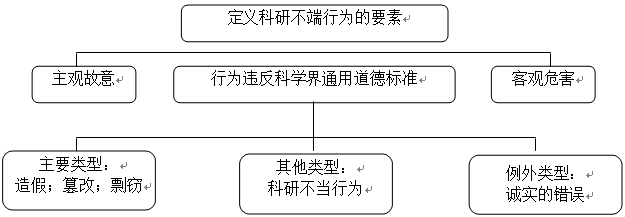
\includegraphics[width=12cm]{images/chapters/5.1}
	\caption{科研不端行为的理解} 
	\label{fig:5.1} 
\end{figure}

2)损害他人著作权,包括:侵犯他人的署名权,如将做出创造性贡献的人排除在作者名单之外,未经本人同意将其列入作者名单,将不应享有署名权的人列入作者名单,无理要求著者或合著者身份或排名,或未经原作者允许用其他手段取得他人作品的著者或合著者身份。剽窃他人的学术成果,如将他人材料上的文字或概念作为自己的发表,故意省略引用他人成果的事实,使人产生为其新发现、新发明的印象,或引用时故意篡改内容、断章取义。

3)违反职业道德利用他人重要的学术认识、假设、学说或者研究计划,包括:未经许可利用同行评议或其它方式获得的上述信息;未经授权就将上述信息发表或者透露给第三者;窃取他人的研究计划和学术思想据为己有。

4)研究成果发表或出版中的科学不端行为,包括:将同一研究成果提交多个出版机构出版或提交多个出版物发表;将本质上相同的研究成果改头换面发表;将基于同样的数据集或数据子集的研究成果以多篇作品出版或发表,除非各作品间有密切的承继关系。

5)故意干扰或妨碍他人的研究活动,包括故意损坏、强占或扣压他人研究活动中必需的仪器设备、文献资料、数据、软件或其他与科研有关的物品。

6)在科研活动过程中违背社会道德,包括骗取经费、装备和其他支持条件等科研资源;滥用科研资源,用科研资源谋取不当利益,严重浪费科研资源;在个人履历表、资助申请表、职位申请表,以及公开声明中故意包含不准确或会引起误解的信息,故意隐瞒重要信息。

\subsection{科研不端行为的表现形式}

从表现形式看,有三类科研不端行为,即杜撰、篡改、剽窃(FFP)。

\textbf{1)杜撰(fabrication)}

杜撰一般指按照某种科学假说和理论演绎出的期望值伪造虚假的观察与实验结果,从而支持理论的正确性或者确认实验结果的正确性。它表现为对科学和实验结果的不尊重,按照个人主观意愿无中生有,捏造事实。

按照科研的内容和程序分类,杜撰主要分两种:第一,科研申请中的杜撰。主要指在项目资金申请、科研成果申报,以及职位申请等其他科研活动中做虚假的陈述,如杜撰学历、杜撰论文或书刊发表记录、提供虚假获奖证书、文献引用证明,等等;第二,科研过程中的杜撰。主要指在科研过程中,未经过试验、调查,仅根据局部科学现象甚至根本没有根据,凭空编造、虚拟出一些试验数据、结果或事实、证据来作为支持自己论点的论据,证明某理论的正确性。而凭空编造出来的数据或实验结果不具有可重复性,与真实的数据互不兼容。

\textbf{2)篡改(falsification)}

篡改,主要是指在科研过程中,用作伪的手段按自己的期望随意改动、任意取舍原始数据或试验使得结果符合自己的研究结论、支持自己的论点。

篡改数据违背了科研规范中的一个基本要求,就是要忠实的记录和保存原始数据。用个人主观意愿对科研结果横加干预,其实验结果必然不具有可重复性。

篡改行为的表现形式主要包括两种:第一,篡改数据,主要指以一些实验结果为基础推测实验结果,对另一些与推测其他结果不同的实验结果、实验记录和图片进行修改。第二,拼凑数据,主要指按期望值主观取舍、任意组合实验结果,或者把与期望值不符的实验结果删除,只保留与期望值一致的实验结果。

\textbf{3)剽窃((plagiarism)}

剽窃是指将他人的科研成果或论文全部或部分原样照抄,并以自己名义发表的欺诈行为。它不仅包括对他人作品字句、内容的直接使用,也包括对他人学术论著的思想、观点、结构、体系等元素作为自己论著的基本元素加以使用并发表的行为。通常表现为不尊重他人学术思想、学术观点,不注明学术思想、学术观点的出处来源而随意使用。

在学术研究中,对已有成果的了解是必需的,对已有成果的借鉴也是不可避免的,因此是否适当引用就成为判断剽窃或借鉴的关键。正确的引用包括两个方面的含义:一是凡借鉴就要引用,引用就要对原出处进行明示;二是引用只能反映研究者对本研究领域已有研究成果的了解和借鉴,或反映已有成果与自己研究的关系,不能构成自己研究成果的主体内容。

\section{科研不当行为}

本节内容均摘自文献[3]。

\subsection{科研不当行为的定义}

科研不当行为(questionable research practice,QRP)是指虽然违反科学的目的、精神和科学研究事业的基本道德原则,但没有直接触犯明确规定的研究活动的道德底线的行为。

科研不当行为的特征主要为:第一,科研不当行为以明确不违反科学共同体规约为前提,更不是一种违法行为。第二,科研不当行为虽然不是科学共同体规约所明确禁止,但它是不合理的,具有不合理、不公正、不合乎科学道德的特征。

\subsection{科研不当行为的表现形式}

科研不当行为的表现形式很多,一般来说,科研不当行为主要可分为五种类型:

\textbf{1)数据的不当使用}

(1) 根据本能感觉,排除本人认为不精确的观测或数据点;或因匆忙完成项目而偷工减料;

(2)未能在合理的期间内获得重要研究数据;

(3)维持不充分的研究记录,特别是那些用于发表或被他人所依赖的结果;

(4)运用不恰当的统计学或其他计量方法提高研究结论的重要性;

(5)在论文中给出理由的情况下将异常值从数据集中剔除;

(6)为了提高研究的重要性,运用不恰当的统计方法;

(7)窃取供应品、书籍或数据;

(8)操纵实验以获得本人想要的结果;

(9)未经许可复制数据、论文或软件程序;

(10)在合理的期间内,未能保持良好的研究记录或研究数据。

\textbf{2)违反科学规则}

(1)忽视材料处理政策的细节(如生物安全、放射性材料等);运用一个项目的资金完成其他项目;

(2)在人体研究实验中没有报告不良事件;

(3)在研究中不珍惜动物资源;

(4)违反本人所在研究机构的生物安全规定而未尽告知义务,将员工和学生暴露于生物风险之中。

\textbf{3)不当的同行关系则}

(1)通过与论文研究无重要关联的特殊服务获取署名;

(2)在同事没有对论文作出重大贡献的情况下将其列为作者,以作为人情回报;

(3)为了确保本人成为唯一的发明人,未告知合作者本人申请专利的意图;

(4)未经授权运用他人的想法,或对这种使用未给予应有的感谢;

(5)与同事讨论本人所正在承担的期刊论文审稿工作中获得的保密数据;

(6)规避同行审查程序并通过媒体发布会公布本人的研究结果,而未给予同行足够的时间评估本人的工作;

(7)在文献综述中未能表明在该领域的其他人或相关前期工作的贡献;

(8)妨害他人的工作;

(9)评审他人论文时未经认真阅读即拒绝论文的发表;

(10)在评审工作中做出贬损的评论乃至贬损他人人格;

(11)拒绝同行接触作为已发表论文之支撑的独一无二的研究材料或数据。

\textbf{4)不当的师生关系}

(1)基于财、物、性等交易行为许诺学生以更好的成绩;

(2)过度使用、忽略或剥削研究生或博士后的劳动;

(3)提供过于正面或过于负面的推荐信。

\textbf{5)基于产出压力的不当科研}

(1)在基金项目的申请中夸大事实,以说服评审人此项目将会对该领域做出重大贡献;

(2)为了应对资助方的压力,修改研究的设计、方法或者结果;

(3)在论文或计划中保留方法或结果的细节;

(4)将推测歪曲为事实或者公布初步的研究结果(特别是在大众媒体上),而未能提供充分的数据使得同行可以评判结果的有效性或重复该实验;

(5)在两种或两种以上不同的期刊上发表相同的论文,而未告知编辑,即一稿多投或一稿多发;

(6)在工作申请或建立中夸大事实;

(7)在资助本人研究的公司中拥有实质性数量的股份而未披露此种经济利益;

(8)故意夸大新药的临床效果以获得经济利益。

\section{科研规范}

本节内容均摘自文献[3]。

科研规范(或学术规范)主要是指从事科研活动的行为规范,是以科研道德为基础,以科学共同体为主体,对科研及其相关行为作出的规制性安排。当代科技工作者应坚持的科研规范包括:诚实原则、公开原则、公正原则、尊重知识产权、声明与回避原则。

\subsection{研究数据收集、记录和保存中的规范}

数据直接影响到研究成果,因此应当从源头上抓好数据的规范行为。

在数据收集过程中,首先应保证获得数据的条件是真实的,而不是虚构的;其次要确保收集和保存实验数据的完整性;第三,不能为某种目的或获取利益对原始数据进行人为加工和篡改;第四,收集特殊数据应当事先获得授权许可。

数据记录应当与数据的获得同步。数据记录必须精准,必须严格按照有关程序和规则记录数据。

在数据保存方面,第一,应以严谨的方式保存数据。如果是书面记录,就要存放在安全的地方;如果是计算机文件,就应备份,并注意将备份的数据保存在安全处,备份数据应与原始数据分开保存,并且定期为所保存的数据重新备份。第二,原始数据应由产生这些数据的研究机构和科研人员共同保存。第三,要慎重保存涉及机密或危险的数据。第四,应做好数据保存相关事项的预先协议。第五,遵守数据保存期限但不应有意隐蔽数据。

\subsection{研究数据使用中的规范}
在未通过发表物或公开宣布研究成果而确立优先权之前,科研人员可以独自使用已经得到确证或有效的数据。一旦科研人员将实验结果公开发表,其他人就可以自由地获取实验涉及到的所有数据,包括最终结果,以便于检验和使用。

在数据使用和处理成图像过程中,首先,应当保证原始数据的真实性,并且保证图像是对数据的真实体现;其次,论著中的数据图像必须是原始记录的完整体现;第三,他人制作完成的数据图像应当在论著中予以说明;第四,应当熟知和合理运用现有相关处理数据的计量方法;第五,应当预先了解拟投稿的相关出版社或期刊的数据和图像处理规范或相关指南;第六,应当了解哪些行为是会受到处罚,以及将会受到怎样的处理。


\subsection{引文的规范}

\section{本章小结}
介绍了科研不端行为和科研不当行为以及科研规范。











\chapter{参考文献的标注和要求}

学位论文必须要列参考文献,以说明著述内容的科学根据和出处,进而方便读者扩展性阅读的查找。若引用他人成果,应列出引文出处,以尊重他人的科学研究成果[2,15]。\textcolor{red}{(注:仅参考此格式进行排版。参考文献具体格式及排版见后面“参考文献”部分。)}

\section{参考文献的重要性}

参考文献反映论文作者的科学态度和论文具有真实、广泛的科学依据,也反映论文的起点和深度。方便论文作者与前人的成果区别开来,是对他人劳动成果的尊重。方便读者检索和查找有关资料。有利于节省论文篇幅,有助于科技情报人员进行情报研究和计量学研究。

\section{顺序编码体系}

参考文献标著录有如下4种体系:著者-出版年体系(Harvard体系),顺序编码体系,数字字母混合体系和出版年顺序体系[4]。我校本科学位论文的参考文献标注采用顺序编码体系。即参考文献以文献在整个学位论文中出现的次序用[1]、[2]、[3]…形式统一排序、依次列出,置于文中提及的文字末尾的右上角,视引文表标注情况,置于标点符号前或后[4]。

\subsection{正文中引用文献的标注方法}

正文中引用文献的标示应置于所引内容最后一个字的右上角,所引文献编号用阿拉伯数字置于方括号“[ ]”中,用小4号字体的上角标,引用单篇文献时如例1所示;引用两篇文献时,各篇文献序号置于同一个方括号内,其间用逗号(不是顿号)分开,如例2所示,如果连续序号多于两个以上时,可用范围号“~”(中文还可用全身“—”,外文用en-dash“-”)连接起讫序号,如例3所示;如果文献序号作为叙述文字的一部分,则文献号与正文平排,并且每条文献都要加方括号,如例4和例5所示;如果同一文献在文中不同处被重复引用,全文只在其第一次出现时标应标的序号,以后各处均标这同一序号;若必须标出引文页码,可把页码标在方括号外,如例6所示,也可用其他明确的方式标出。

例1:……,表明已低到2500 m的高度[2],……。

例2:原位生成的TiB主要有针状或晶须状[21,22]

例3:复杂网络是当今学术界的研究热点[3-6],早期的研究结果[2,4,6-9] 表明,……。

例4:文献[2]指出,此高度已低到2500 m。

例5:紫色土壤主要分布在我国西南地区(参见文献[11]、[12]、[32])。

例6:……,表明已低到2500 m的高度[2,35],……。

不得将引用文献标示置于各级标题处。


\subsection{文后参考文献表的著录方法}


按论文中引用的顺序号排列参考文献,不按著者,不分语种。多著者时,著者间用西文逗号隔开,只列前3人,后加“等(et al.)”。在句中,凡是西文符号后应空半格。

参考文献的著录格式严格按照以下形式书写(含标点符号):

\textbf{1)专著:}作者.书名.版本(第1版不著录)[M].出版地:出版者,出版年:引用起止页码.

\textbf{2)译著:}作者.书名[M].译者,译.出版地:出版者,出版年: 引用起止页码.

\textbf{3)期刊:}作者.题名[J].刊名,出版年份,卷(期):起止页码.

\textbf{4)会议论文集:}作者.题名[C]// 编者.论文集名.出版地:出版者,出版年:起止页码.

\textbf{5)学位论文:}作者.题名:[D].保存地:保存者,年份.

\textbf{6)专利文献}:专利申请者.题名.专利国别,专利号[P].公告日期或公开日期.

\textbf{7)标准:}责任者.标准代号标准名称[S].出版地:出版者,出版年.

\textbf{8)电子文献标注格式:}主要责任者.题名: 其它题名信息[文献类型标志/文献载体标志].出版地: 出版者, 出版年(更新或修改日期)(引用日期).获取和访问路径.

参考文献著录时还应注意:参考文献中的外文作者名、外文刊名的缩写一律不用缩写点。外文著者一律用姓在名前,采用首字母缩写(中国人用全名不缩写)。姓和名之间不加逗号,名2个以上大写首字母,2名间空一格。文献作者3名以内全部列出,4名以上则列前3人,后加“et al”。各著者间不加“and”、“和”等,应用逗号分开。外文题名第一个单词首字母大写,其余单词(专有名词除外)均不大写。外文刊名应按国际标准规定缩写,不加缩写点。

特别提醒,对西文作者,正文中引用时应遵循西文规范,即名在前姓在后,缩写部分要加缩写点。以参考文献[10]为例,其参考文献条目为:

[10]\quad Atzori L, Iera A, Morabito G. The internet of things: a survey[J]. Computer Networks, 2010, 54(15): 2787 -2805.

正文中引用时的文字为:“L. Atzori等人对物联网的进展进行了综述,指出……”。西文人名乱用、不当使用是常见的写作问题。

通过查非发现,大部分论文参考文献格式都存在各种问题,应该严格规范执行。更多样例见本模板参考文献部分。如有未尽之处,可参看发表的重邮学报论文参考文献标注样例。需要特别说明的是,由于不是所有已发表论文或高年级撰写的学位论文都严格执行了同一规范,请勿将不规范的格式当做模仿对象,以免给自己带来后续问题。

\section{参考文献要求}

1)所有被引用文献均要列入参考文献中,必须按顺序标注,但同一篇文章只用一个序号。

2)参考文献数量不得少于15篇,各二级学院应按不同专业提出外文参考文献具体要求,教科书和硕士学位论文不得多于5本,其中外文文献不少于5条。参考文献中近三年的文献数一般应不少于总数的1/3,并应有近两年的参考文献。(网上参考文献和各类标准不包含在上述规定的文献数量之内)。

3)教材、产品说明书、未公开发表的研究报告(著名的内部报告如PB、AD报告及著名大公司的企业技术报告等除外)等通常不宜作为参考文献引用。一些未公开发表的内容引用时,可以采用注释如脚注的方式。

4)引用网上参考文献时,应注明该文献的准确网页地址。因为网上文献大都不规范,除特殊情况,原则上不引用,尽量用脚注方式给出。如测试数据来源网址,在正文首次出现时均可直接脚注或正文中给出出处。

5)序号应按文献在论文中的被引用顺序编排。换行时与作者名第一个字对齐。若同一文献中有多处被引用,则要写出相应引用页码,各起止页码间空一格,排列按引用顺序,不按页码顺序。

参考文献内容中文宋体,英文Times New Roman,小4号宋体,1.5倍行距。

Word也提供了参考文献引用的基本功能,但维护一致性比较困难。目前有较多的参考文献管理软件或工具,各有利弊,可根据情况使用,相互交流使用经验,更好地做好文献管理。

\section{本章小结}

介绍了参考文献的标注方法、著录方法和相关要求。











\chapter{总结与展望}

学位论文应有结论,可以从论文的主要工作、创新点和后续的研究工作等方面进行总结。\textcolor{red}{(注:仅参考此格式进行排版。)}

\section{主要工作与创新点}

学位论文的结论是最终的、总体的结论,不是正文中各段的小结的简单重复。结论应该观点明确、严谨、完整、准确、精炼。文字必须简明扼要。可以从论文的主要工作、创新点和后续的研究工作等方面总结。

如果不可能导出应有的结论,也可以没有结论而进行必要的讨论。

可以在结论或讨论中提出建议、研究设想、仪器设备改进意见、尚待解决的问题等。不要简单重复罗列实验结果,要认真阐明本人在科研工作中创造性的成果和新见解,在本领域中的地位和作用,新见解的意义。对存在的问题和不足应作出客观的叙述。应严格区分自己的成果与他人(特别是导师的)科研成果的界限。

一般应按四级标题的方式给出,根据需要设置数量。如本文主要工作和创新点如下:

1)阐述第一个创新工作。不要把阅读文献当成创新工作。

2)阐述第二个创新工作。

3)阐述第三个创新工作。

4)阐述第四个创新工作。

特别提醒,不应简单和中文摘要内容相互拷贝。同一段文字或句子在本文中原则上只出现一次。

\section{后续研究工作展望}

针对工作不足或问题,说明更下一步深入的研究。如内容较多,也应用四级标题方式列出。

\newpage\quad %加一页,使得参考文献第一页的页眉为 参考文献
\backmatter
%================================
% 参考文献
%参考文献是毕业设计(论文)不可缺少的组成部分,它反映论文作者的科学态度和毕业设计(论文)的取材来源、广博程度和可靠程度,同时能方便地把作者的研究成果与他人的成果区别开来。一份完整的参考文献也是向读者提供的一份有价值的信息资料。参考文献应列入主要的中外文献,数量不少于15篇,教科书和硕士论文不多于5本。按论文中参考文献出现的次序,用中括号以数字连续编号,格式参考毕业设计(论文)模版。
% 参考文献使用
% 设置参考文献风格,参照使用 https://github.com/Haixing-Hu/GBT7714-2005-BibTeX-Style
% TeX技巧/参考文献 https://www.latexstudio.net/archives/1541.html
% TeX技巧/参考文献需要注意的一些小问题 https://blog.csdn.net/jialiyk/article/details/124990632
% 参考文献呈现方式
\bibliographystyle{reference/gbt7714-2005}
% .bib文件名  此参考文献在文件夹reference下,名为ref.bib文件
\bibliography{reference/ref}
\newpage\quad %加一页,使得致谢第一页的页眉为 致谢


% 致谢
%% 致谢

\chapter{致谢}
{\songti\xiaosi
致谢二字一级标题:黑体3号字居中,段前17磅,段后16.5磅,1.5倍行距,致谢二字与致谢内容之间不空行。致谢内容正文样式:宋体小四号,1.5倍行距。

可以从下列方面致谢:协助完成研究工作和提供便利条件的组织或个人;在研究工作中提出建议和提供帮助的人;给予转载和引用权的资料、图片、文献、研究思想和设想的所有者;其他应感谢的组织或个人。

主要感谢导师和对论文工作有直接贡献及帮助的人士和单位。学位申请人的家属及亲朋好友等与论文无直接关系的人员,一般不列入致谢的范围。

致谢辞应谦虚诚恳,实事求是,切忌浮夸与庸俗之词。 }

\newpage\quad %加一页,使得附录A第一页的页眉为 附录A

% 附录
%% 附录页

\chapter{附录A\quad 科技写作中非学术型低级错误的主要表现}

本附录主要针对学位论文写作或中文科技论文写作,供重庆邮电大学学位论文查非工作参考。未尽事宜,可参考重庆邮电大学论文写作要求、重庆邮电大学学报编辑部等国内期刊社、出版社的通用出版规定。

推荐阅读《科学出版社作者编辑手册》、《科学道德与学风建设宣传参考大纲(试用本)》等写作指导性书籍或资料,可了解更多、更详尽的通用写作出版规范。

\textcolor{red}{(注:对于一些不宜放入正文中,但作为毕业设计(论文)又不可缺的组成部分或具有重要参考价值的内容,可编入毕业设计(论文)的附录中,例如,公式的推演、源程序代码、附图等内容。附录的内容为备选项目,作者可根据内容的需要决定附录的项目数,用附录A、附录B方式编号。附录的篇幅不宜太多。附录与主体部分一起编制页码。若附录部分有手工制作或复印件,手工制作或复印件部分要装订在内但可以不计页码。附录的文字按照正文格式进行排版。)}

\textcolor{red}{(附:科技写作中非学术型低级错误的主要表现见 moban文件夹下)}

\textbf{代码效果演示:}
\begin{python}
# 这是一段代码测试
def CQUPT():
    print("Hello,CQUPT")
    print("学长学长,给咱们讲讲3G芯片的故事呗。")
    print("这是世界上第一枚0.13微米工艺的TD-SCDMA 3G手机基带芯片。"
         +"它的诞生,标志着我国3G通信核心芯片等关键...")
CQUPT()
\end{python}
\newpage\quad %加一页,使得附录B第一页的页眉为 附录B


%% 附录页


\chapter{附录B\quad 英文翻译}
% \addcontentsline{toc}{chapter}{附录}

\textcolor{red}{指导教师制定与专业相关的外文文献内容,由学生独立翻译成中文,其外文文献内容翻译成中文后的内容不得少于3000字符。译文和原文附于附录部分,按照正文格式进行排版。若原文没有电子版只是原版的复印件,复印件装订在内可不计页码。}
%================================
\end{document}
